\subsection{Opgave 12}
To ensvinklede trekanter er vist på figuren.\\\\
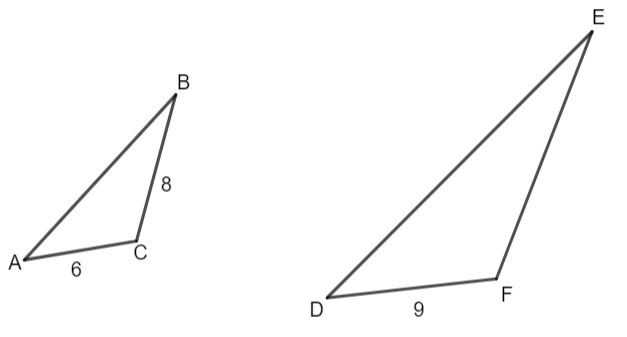
\includegraphics[width=10cm]{Opgave_11-20/Opgave_12/Opgave_12.jpg}\\\\
\textbf{Størrelsesforholdene er ikke korrekte.}\\\\

Følgende sidelængder oplyses: $|AC| = 6,\; |BC| = 8$ og $|DF| = 9$\\\\

Bestem $FE|$\\\\

\ans
Da trekanterne er ensvinklede kan vi altså bestemme sidelængdernes størrelsesforhold. Hvis vi ser på sidelængderne $|AC|$ og $|DF|$ er den større trekants side 1.5 gange længere. Vi kan altså bestemme sidelængden $|FE| = 1.5\cdot |BC| = 1.5\cdot 8 = 12$. 